\documentclass[10pt]{beamer}
\usepackage[italian]{babel}
\usepackage[utf8]{inputenc}
\usepackage[T1]{fontenc}
\usepackage{tikz}
\usepackage{pgfplots} % grafici
\usetikzlibrary{shapes,snakes}

% TEMA
%\usetheme{EastLansing}
\usetheme{Madrid}
%\usetheme{CambridgeUS}
\usecolortheme{whale}
%\usecolortheme{dolphin}
%\setbeamercovered{transparent}
\beamertemplatenavigationsymbolsempty

% LOGO
%\pgfdeclareimage[height=2cm]{logo}{logo/unifi}
%\logo{\includegraphics[width=1.5cm]{logo/unifi}}
\titlegraphic{\includegraphics[width=1.5cm]{logo/unifi}}

% DATI
\title[Model checking e sistemi adattivi]{Model checking come supporto \\ per le scelte di sistemi adattivi}
\author[Marco Tinacci]{\emph{Marco Tinacci}}
\institute[Unifi]{
	{\normalsize \begin{tabular}{ccc}
		Relatore &\hspace{4cm}& Correlatore \\
		\emph{Rocco De Nicola} &\hspace{4cm}& \emph{Michele Loreti} \\
	\end{tabular}
	}\\[15pt]
Dipartimento di Sistemi e Informatica \\
Università degli Studi di Firenze
}
\date{15 Ottobre 2012}

\begin{document}
	% ===============================================================
	% TITOLO
	% ===============================================================
	\begin{frame}
		\maketitle		
	\end{frame}
	% ===============================================================
	% SOMMARIO
	% ===============================================================
	\section*{Sommario}
	\begin{frame}
		\tableofcontents
	\end{frame}
	% ===============================================================
	% SISTEMA ADATTIVO
	% ===============================================================	
	\section{Sistemi adattivi}
	\begin{frame}
		\frametitle{Definizione di sistema adattivo}
		\begin{block}{\emph{``In che caso un sistema si dice adattivo?''}}
			Un sistema è \emph{adattivo} quando il suo \alert{comportamento} dipende da un insieme di \alert{dati di controllo} che possono variare durante l'esecuzione			
		\end{block}
		\begin{block}{\emph{``Cosa si vuole ottenere tramite l'adattività?''}}
			Si vuole elaborare una \alert{strategia} che permetta al sistema di raggiungere il suo \alert{obiettivo}
		\end{block}
		\begin{block}{\emph{``Perché usare un approccio adattivo?''}}
			Questo approccio risulta utile in situazioni dove il sistema ha una conoscenza parziale o nulla dell'\alert{ambiente}
		\end{block}
	\end{frame}
	
	\begin{frame}
		\frametitle{Esempio - marXbot}
		\begin{columns}
			\begin{column}{0.6\textwidth}
				Sensori
				\begin{itemize}
					\item sensori di prossimità
					\item sensori di luce
					\item videocamere
				\end{itemize}
				Attuatori
				\begin{itemize}
					\item ruote
					\item led luminosi
					\item dispositivi di connessione
				\end{itemize}
				Ciclo di feedback
				\begin{itemize}
					\item controllo - \alert{dati di controllo}
					\item elaborazione - \alert{strategia}
					\item attuazione - \alert{comportamento}
				\end{itemize}
			\end{column}
			\begin{column}{0.4\textwidth}
				\includegraphics[width=0.7\textwidth]{Images/marxbot}
			\end{column}
		\end{columns}
	\end{frame}
	% ===============================================================
	% MODEL CHECKING
	% ===============================================================	
	\section{Model checking}
	\begin{frame}
%		\frametitle{Model checking}
		\begin{block}{Model checking}
			Il \emph{model checking} è un metodo di verifica formale di un modello
		\end{block}
		\begin{center}
		\begin{tikzpicture}[scale=.7]
			\tikzstyle{block} = [draw, rectangle, minimum height=2em, minimum width = 4em, thick, scale=.7]
			\tikzstyle{data} = [draw, ellipse, minimum height=2em, minimum width = 4em, scale=.7]

%			\draw[help lines] (0,0) grid (4,5);
			
			\onslide<1-4>{\draw (0,5) node[data, name=req] {Requisiti};}
			\draw (4,5) node[data, name=sis] {Sistema};
			\draw (2,2) node[block, name=mc] {Model checker};

			\draw (0,1) node[data, name=sat] {Soddisfatto};
			\draw (4,1) node[data, name=con] {Controesempio};
			\draw[->] (mc) -- (sat);
			\draw[->] (mc) -- (con);

			\onslide<1>{
				\draw[->, dashed] (req) -- (mc);
				\draw[->, dashed] (sis) -- (mc);
			}
			
			\onslide<2->{\alert<2>{
				\draw node[block, name=form, below of=req] {Formalizzazione};
				\draw node[data, name=prop, below of=form] {Proprietà};
				\draw[->] (form) -- (prop);
				\draw[->] (prop) -- (mc);
			}}
			
			\onslide<2-4>{
				\alert<2>{\draw[->] (req) -- (form);}
			}
			
			\onslide<2->{\alert<2>{
				\draw node[block, name=model, below of=sis] {Modellazione};
				\draw[->] (sis) -- (model);
				\draw node[data, name=modello, below of=model] {Modello};
				\draw[->] (model) -- (modello);
				\draw[->] (modello) -- (mc);
			}}
			\onslide<3->{\alert<3>{
				\draw (2,0) node[data, name=mem] {Memory overflow};
				\draw[->] (mc) -- (mem);
				\draw[->] (con) -- (6,1) -- (6,4) -- (model);
			}}
			
			\onslide<5->{
				\draw (-1.5,5) node[data, name=req2] {Requisiti};
				\draw[->] (req2) -- (form);
				\alert{
					\draw (1.2,5) node[data, name=acc] {Accuratezza};
					\draw[->] (acc) -- (form);
				}
			}
		\end{tikzpicture}
		\end{center}
		\onslide<4->\begin{block}{Esempio di proprietà}
			I messaggi scambiati tra due terminali vengono trasmessi correttamente
		\end{block}
		\onslide<5>\begin{block}{Esempio di proprietà quantitativa}
			I messaggi scambiati tra due terminali vengono trasmessi correttamente con una probabilità maggiore di $0.99$
		\end{block}
	\end{frame}

%	\begin{frame}
%		\frametitle{PRISM}
%		\begin{block}{}
%			\emph{PRISM} è un model checker che presenta le seguenti caratteristiche:
%			\begin{itemize}
%				\item permette di definire modelli con aspetti \emph{nondeterministici} e \emph{probabilistici} tramite un linguaggio specifico
%				\item permette di formalizzare le proprietà tramite formule \emph{PCTL}
%			\end{itemize}
%		\end{block}
%	\end{frame}
	
	\begin{frame}
		\frametitle{Problema: come risolvere le scelte?}
		\begin{exampleblock}{Idea}
		Utilizziamo il model checking all'interno del criterio di risoluzione delle scelte
		\end{exampleblock}
		\begin{center}
		\begin{tikzpicture}[scale=.6]
			\tikzstyle{block} = [draw, rectangle, minimum height=2em, minimum width = 4em, thick, scale=.6]
			\tikzstyle{data} = [draw, ellipse, minimum height=2em, minimum width = 4em, scale=.6]
%			\draw[help lines] (0,0) grid (4,5);
			\draw (0,2) node[data, name=prop] {Proprietà};
			\draw (4,2) node[data, name=mod] {Modello};
			\draw (2,1) node[block, name=mc] {Model checker};
			\draw (0,0) node[data, name=sat] {Soddisfatto};
			\draw (4,0) node[data, name=con] {Controesempio};
			\draw[->] (prop) -- (mc);
			\draw[->] (mod) -- (mc);
			\draw[->] (mc) -- (sat);
			\draw[->] (mc) -- (con);

			\onslide<2>{\alert{
				\draw (4,3) node[data, name=hp] {Ipotesi};
				\draw[->] (hp) -- (mod);
			}}
			
			\onslide<3>{
				\draw (4,3) node[data, name=hp] {Ipotesi};
				\draw[->] (hp) -- (mod);			
				\alert{
					\draw (0,3) node[data, name=obj] {Obiettivo};
					\draw[->] (obj) -- (prop);
				}
			}
			
			\onslide<4->{
				\draw (4,3) node[data, name=hp] {Ipotesi};
				\draw[->] (hp) -- (mod);
				\draw (0,3) node[data, name=obj] {Obiettivo};
				\draw[->] (obj) -- (prop);
			}
		\end{tikzpicture}
		\end{center}
		\onslide<2->{
			\begin{itemize}
				\onslide<2->\item le lacune sulla conoscenza dell'ambiente vengono colmate da \alert{ipotesi}
				\onslide<3->{\item 
					come proprietà da verificare viene data una formula che descrive l'\alert{obiettivo} del sistema che deve prendere le decisioni
				}
				\onslide<4->{\item 
					il model checker viene usato in un modo non convenzionale per fare \alert{previsioni} invece che verifiche
					}
				\onslide<5->{\item 
				viene valutato l'esito delle previsioni per ogni stato del modello raggiungibile da una scelta dell'agente principale, la decisione da prendere è quella che porta alla più alta probabilità di successo
					}
			\end{itemize}
		}
	\end{frame}
	% ===============================================================
	% LAPSA
	% ===============================================================	
	\section{LAPSA: un linguaggio per popolazioni di agenti adattivi}
	\begin{frame}
		\frametitle{LAPSA: Language for Population of Self-adaptive Agents - 1}
Impone la visione dell'agente principale consentendo di descrivere le ipotesi che si fanno sull'ambiente
		\begin{block}{Programma LAPSA}
		$$
		\begin{array}{rcl}
			\mathit{program} &::=& \mathbf{subject} \ \mathit{module} \\
				&& \mathit{modules} \\
				&& \mathit{environment} \\
		\end{array}
		$$
		\end{block}
		\begin{center}
			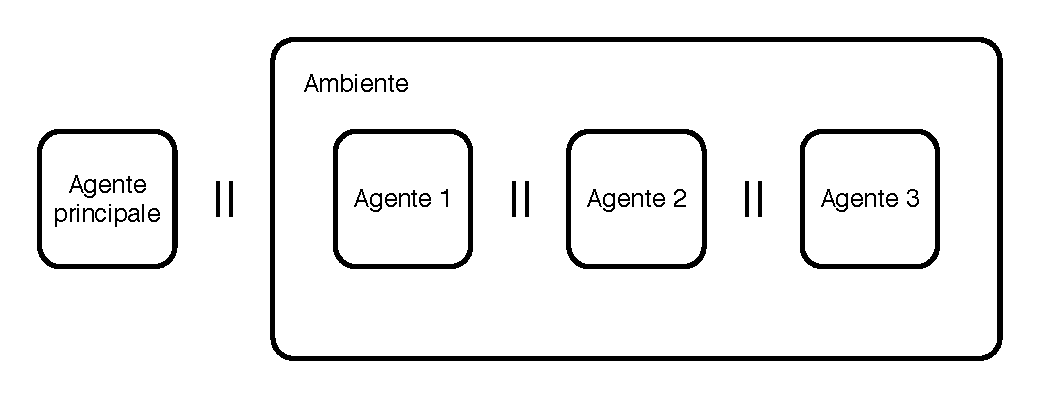
\includegraphics[width=.7\textwidth]{Images/schemaidea}
		\end{center}
	\end{frame}
	
	\begin{frame}
		\frametitle{LAPSA: Language for Population of Self-adaptive Agents - 2}
		%È un linguaggio che permette di definire sistemi \alert{reattivi}
		\begin{block}{Modulo}
			$$ \mathit{module} ::= \mathbf{module} \ \sf{module}\textrm{-}\sf{id} \ \{ \mathit{variables} \ \mathit{rules} \ \mathit{targets} \} $$
		\end{block}
		\begin{block}{Transizione}
		$$
		\mathit{rules} ::= \mathit{condition} \Rightarrow \mathit{distribution}; \quad|\quad \mathit{rules} \ \mathit{rules}
		$$
		\end{block}
		\begin{block}{Obiettivo}
		$$
		\begin{array}{rcl}
			\mathit{targets} ::= \mathbf{target} \ \mathit{condition} \quad|\quad \mathit{targets} \ \mathit{targets}
		\end{array}
		$$
		\end{block}
	\end{frame}
	\begin{frame}
		\frametitle{LAPSA: Language for Population of Self-adaptive Agents - 3}
		\begin{block}{Condizione}
		$$
		\begin{array}{rcl}
	\mathit{condition} &::=& \ \mathbf{exists} \ \sf{variable}\textrm{-}\sf{id}:\sf{module}\textrm{-}\sf{id} \ \mathbf{such}\ \mathbf{that} \ \mathit{condition} \\
	&|& \mathit{expression} \bowtie \mathit{expression} \quad|\quad \mathit{condition} \ \mathbf{or} \ \mathit{condition} \\
	&|& \mathbf{not} \ \mathit{condition} \quad|\quad (\mathit{condition}) \quad|\quad \mathbf{true} \\
		\end{array}
		$$
		\end{block}
		\begin{exampleblock}{Esempio di quantificatore esistenziale}
			$$ \mathbf{exists}\ r\ :\ robot\ \mathbf{such}\ \mathbf{that}\ r.x > 3 $$
		\end{exampleblock}
		\begin{block}{Distribuzione}
		$$		
		\mathit{distribution} ::= <\mathit{expression}> \mathit{update} \quad|\quad \mathit{distribution} \ \# \ \mathit{distribution}
		$$
		\end{block}
		\begin{exampleblock}{Esempio di distribuzione}
			$$ <1> x=x+1 \ \# \ <2> x=x-1 $$
		\end{exampleblock}
	\end{frame}
	\begin{frame}
		\frametitle{Compilatore LAPSA}
		\begin{itemize}
			\item implementazione in \alert{Java}
			\item plugin di Eclipse tramite \alert{Xtext}
			\item utilizza \alert{PRISM}, un model checker probabilistico
			\item usa una \alert{logica temporale} per definire le formule di proprietà
			\item il risultato è un insieme di probabilità associate a stati che quantificano la possibilità di successo
		\end{itemize}
		\begin{center}
			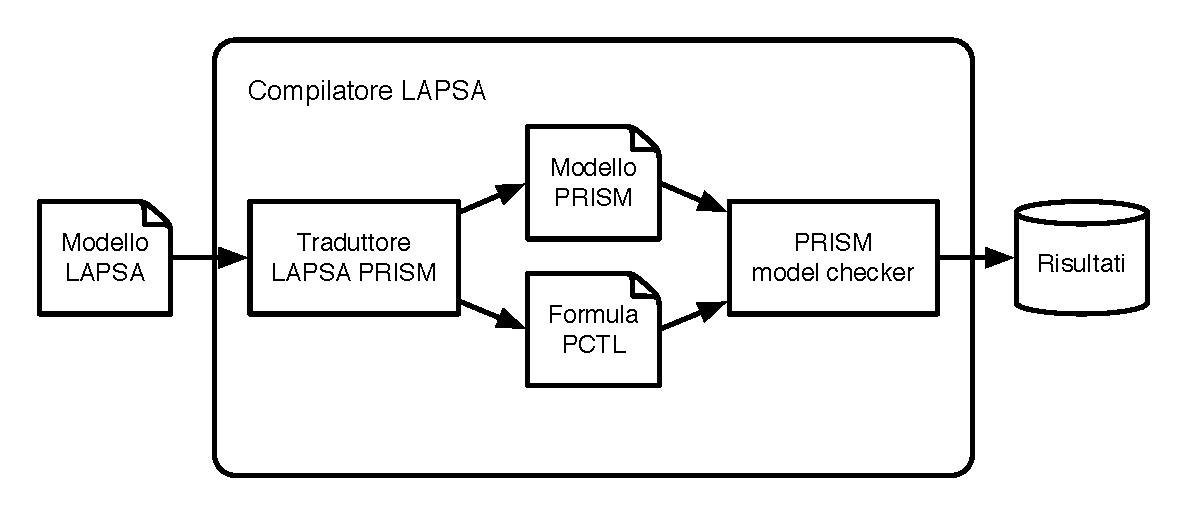
\includegraphics[width=.7\textwidth]{Images/lapsa}
		\end{center}
		
	\end{frame}
	% ===============================================================
	% CASO DI STUDIO
	% ===============================================================	
	\section{Un semplice caso di studio}
	\begin{frame}
		\frametitle{Scenario}
		Lo scenario analizzato è un'arena quadrata contenente una popolazione di marXbot
		\begin{center}
		\begin{tikzpicture}[scale=0.4]
		\begin{scope}
		  \filldraw [fill=gray!10] (4,4) circle (1.4);
	
		  \draw[dashed] (1, 1) grid (5, 5);
		  \draw[very thick, scale=6] (0, 0) grid (1, 1);
	
		  \filldraw [fill=blue!50] (4,4) circle (0.2);
		
		  \filldraw [fill=red!50] (5,5) circle (0.2);
		  \filldraw [fill=red!50] (3,4) circle (0.2);
		  \filldraw [fill=red!50] (2,3) circle (0.2);
		  \filldraw [fill=red!50] (1,2) circle (0.2);
		  \filldraw [fill=red!50] (4,1) circle (0.2);
		  \filldraw [fill=red!50] (2,5) circle (0.2);
		\end{scope}
		\end{tikzpicture}
		\end{center}
		\begin{itemize}
			\item il cerchio blu è il robot principale, quelli rossi sono secondari
			\item l'obiettivo del robot blu è di minimizzare gli scontri con altri robot
			\item tutti i robot possono scegliere periodicamente di muoversi di un passo a nord, sud, ovest o est o di stare fermi
			\item il cerchio grigio rappresenta l'area visibile dal robot blu
			\item i robot rossi si muovono casualmente
		\end{itemize}
	\end{frame}
	\begin{frame}
		\frametitle{Descrizione approccio}
		L'approccio utilizzato può essere riassunto nei seguenti passi
		\begin{enumerate}
			\item scrittura del programma LAPSA
			\begin{itemize}
				\item si ipotizza la presenza di robot che si muovono casualmente
				\item si astrae da tutti i dati esterni all'area visibile dal robot principale
			\end{itemize}
			\item compilazione
				\begin{itemize}
					\item si ottiene una tabella hash che associa ad ogni stato la rispettiva probabilità di successo
				\end{itemize}
			\item scrittura dello scheduler del robot principale che utilizza la tabella hash per ricavare la decisione migliore ad ogni passo
		\end{enumerate}
	\end{frame}

	
	\begin{frame}
		\frametitle{Risultati}
		I risultati sono stati mediati su 300 simulazioni di 100 passi e confrontati con quelli ottenuti da uno scheduler semi-casuale
			\begin{itemize}
				\item per le popolazioni composte da un massimo di 3 robot secondari in un'arena $5\times 5$ il numero di scontri con il robot principale viene diminuito almeno del $20\%$ rispetto a uno scheduler semi-casuale
				\item per una popolazione di 40 robot secondari in un'arena $10\times 10$ il numero di scontri con il robot principale viene diminuito del $31\%$ rispetto a uno scheduler semi-casuale
			\end{itemize}
		% grafico
	\begin{center}
	\begin{tikzpicture}[scale=0.6] %[node distance=0.5cm]
		\begin{axis}[
		enlargelimits=0.15,
		width=0.7*\textwidth,
		ybar,
		ylabel=Collisioni del robot principale,
		xlabel=Dimensione della popolazione,
		symbolic x coords={1, 2, 3, 40},
		xtick=data,
		legend pos= north west
		]
		% semi casuale
		\addplot coordinates {(1,4.22) (2,7.67) (3,11.98) (40,32.86)};
		% model checker
		\addplot coordinates {(1,2.87) (2,6.36) (3,9.82) (40,25.10)};
		\legend{semi-casuale,model checker}
		\end{axis}
	\end{tikzpicture}	
	\end{center}
	\end{frame}
	
	% ===============================================================
	% CONCLUSIONI
	% ===============================================================
	\section{Conclusioni e lavori futuri}
	\begin{frame}
		\frametitle{Conclusioni e lavori futuri}
		\begin{block}{Conclusioni}
		\begin{itemize}
			\item Abbiamo presentato un nuovo approccio per risolvere le scelte di un sistema adattivo
			\item dai risultati abbiamo verificato sperimentalmente la possibilità di un approccio di scelta basato sul model checking
			\item i risultati ottenuti dipendono molto dalle astrazioni e dalle ipotesi che si fanno nel modello LAPSA
		\end{itemize}
		\end{block}
		\begin{block}{Possibili sviluppi futuri}
		\begin{itemize}
			\item estendere LAPSA
			\begin{itemize}
				\item dare memoria agli agenti per permettergli di fare scelte basandosi sulle informazioni ricavate dagli stati precedenti
				\item aggiungere primitive che consentano all’agente di modificare l’ipotesi fatta sull’ambiente
			\end{itemize}
			\item la teoria dei giochi
		\end{itemize}
		\end{block}
	\end{frame}
	
	\begin{frame}
		\begin{block}{}
			\begin{center}
				Grazie per l'attenzione
			\end{center}
		\end{block}
	\end{frame}
	
	% ===============================================================
	% SIMULAZIONE
	% ===============================================================
%	\begin{frame}
%		\frametitle{Simulazione - 1}
%		\begin{columns}
%			\begin{column}{.5\textwidth}
%				Configurazione iniziale, il robot blu è a conoscenza della presenza di altri due robot che si muovono in modo casuale al di fuori della sua area visiva
%			\end{column}
%			\begin{column}{.5\textwidth}
%		\begin{center}
%			\begin{tikzpicture} % 1
%			\begin{scope}
%				\clip (-0.02,-0.02) rectangle (6.02,6.02);
%				\filldraw [fill=gray!10] (1,5) circle (1.4);
%
%				\draw[dashed] (1, 1) grid (5, 5);
%				\draw[very thick, scale=6] (0, 0) grid (1, 1);
%			
%				\draw[->, very thick] (1,5) -- (2,5);
%				\filldraw [fill=blue!50] (1,5) circle (0.2);
%
%				\draw[->, very thick] (1,3) -- (1,4);
%				\filldraw [fill=red!50] (1,3) circle (0.2);
%			
%				\draw[->, very thick] (3,3) -- (3,4);
%				\filldraw [fill=red!50] (3,3) circle (0.2);
%			\end{scope}
%			\end{tikzpicture}
%		\end{center}				
%			\end{column}
%		\end{columns}
%	\end{frame}
%	\begin{frame}
%		\frametitle{Simulazione - 2}
%		\begin{columns}
%			\begin{column}{.5\textwidth}
%		Entrambi i robot rossi sono entrati nell'area visiva del robot blu che decide di rimanere fermo				
%			\end{column}
%			\begin{column}{.5\textwidth}
%		\begin{center}
%		\begin{tikzpicture} % 2
%		\begin{scope}
%			\clip (-0.02,-0.02) rectangle (6.02,6.02);
%			\filldraw [fill=gray!10] (2,5) circle (1.4);
%
%			\draw[dashed] (1, 1) grid (5, 5);
%			\draw[very thick, scale=6] (0, 0) grid (1, 1);
%
%			\filldraw [fill=blue!50] (2,5) circle (0.2);
%
%			\draw[->, very thick] (1,4) -- (2,4);
%			\filldraw [fill=red!50] (1,4) circle (0.2);
%			
%			\draw[->, very thick] (3,4) -- (3,3);
%			\filldraw [fill=red!50] (3,4) circle (0.2);
%		\end{scope}
%		\end{tikzpicture}
%		\end{center}
%			\end{column}
%		\end{columns}
%
%	\end{frame}
%	\begin{frame}
%		\frametitle{Simulazione - 3}
%		\begin{columns}
%			\begin{column}{.5\textwidth}
%		Percependo un altro robot a sud, il robot blu decide di allontanarsi a ovest per evitare un probabile scontro
%			\end{column}
%			\begin{column}{.5\textwidth}
%		\begin{center}
%		\begin{tikzpicture} % 3
%		\begin{scope}
%			\clip (-0.02,-0.02) rectangle (6.02,6.02);
%			\filldraw [fill=gray!10] (2,5) circle (1.4);
%
%			\draw[dashed] (1, 1) grid (5, 5);
%			\draw[very thick, scale=6] (0, 0) grid (1, 1);
%
%			\draw[->, very thick] (2,5) -- (1,5);
%			\filldraw [fill=blue!50] (2,5) circle (0.2);
%
%			\draw[->, very thick] (2,4) -- (3,4);
%			\filldraw [fill=red!50] (2,4) circle (0.2);
%			
%			\draw[->, very thick] (3,3) -- (4,3);
%			\filldraw [fill=red!50] (3,3) circle (0.2);
%		\end{scope}
%		\end{tikzpicture}
%		\end{center}		
%			\end{column}
%		\end{columns}
%	\end{frame}
%	\begin{frame}
%		\frametitle{Simulazione - 4}
%		\begin{columns}
%			\begin{column}{.5\textwidth}
%				Il robot blu rileva la stessa situazione iniziale e prende quindi la stessa decisione di muoversi verso est
%			\end{column}
%			\begin{column}{.5\textwidth}
%		\begin{center}
%		\begin{tikzpicture} % 4
%		\begin{scope}
%			\clip (-0.02,-0.02) rectangle (6.02,6.02);
%			\filldraw [fill=gray!10] (1,5) circle (1.4);
%
%			\draw[dashed] (1, 1) grid (5, 5);
%			\draw[very thick, scale=6] (0, 0) grid (1, 1);
%
%			\draw[->, very thick] (1,5) -- (2,5);
%			\filldraw [fill=blue!50] (1,5) circle (0.2);
%
%			\draw[->, very thick] (3,4) -- (3,5);
%			\filldraw [fill=red!50] (3,4) circle (0.2);
%			
%			\draw[->, very thick] (4,3) -- (3,3);
%			\filldraw [fill=red!50] (4,3) circle (0.2);
%		\end{scope}
%		\end{tikzpicture}
%		\end{center}
%			\end{column}
%		\end{columns}
%	\end{frame}
%	\begin{frame}
%		\frametitle{Simulazione - 5}
%		\begin{columns}
%			\begin{column}{.5\textwidth}
%		Viene nuovamente percepito un robot rosso nelle vicinanze e il robot blu decide di allontanarsi
%			\end{column}
%			\begin{column}{.5\textwidth}
%		\begin{center}
%		\begin{tikzpicture}{scale=.8} % 5
%		\begin{scope}
%			\clip (-0.02,-0.02) rectangle (6.02,6.02);
%			\filldraw [fill=gray!10] (2,5) circle (1.4);
%
%			\draw[dashed] (1, 1) grid (5, 5);
%			\draw[very thick, scale=6] (0, 0) grid (1, 1);
%
%			\draw[->, very thick] (2,5) -- (1,5);
%			\filldraw [fill=blue!50] (2,5) circle (0.2);
%
%			\filldraw [fill=red!50] (3,5) circle (0.2);
%			
%			\draw[->, very thick] (3,3) -- (3,4);
%			\filldraw [fill=red!50] (3,3) circle (0.2);
%		\end{scope}
%		\end{tikzpicture}
%		\end{center}			
%			\end{column}
%		\end{columns}
%	\end{frame}
	
\end{document}